\documentclass[11pt, oneside]{article}   	% use "amsart" instead of "article" for AMSLaTeX format
\usepackage{geometry}                		% See geometry.pdf to learn the layout options. There are lots.
\geometry{letterpaper}                   		% ... or a4paper or a5paper or ... 
\usepackage{graphicx}				% Use pdf, png, jpg, or eps§ with pdflatex; use eps in DVI mode
\usepackage{amssymb}
\title{Homework 6}
\author{Abhi Agarwal}
\date{}

\begin{document}
\maketitle

\par Talked to Tyler Palsulich about this to discuss the ability to declare functions inside SDD. I also talked to him about Question 1.1. My primary mistake was misunderstanding the formats of T1.type, and S2.type and the positions they go in.

\section{Casting}
\subsection*{Question 1.1}
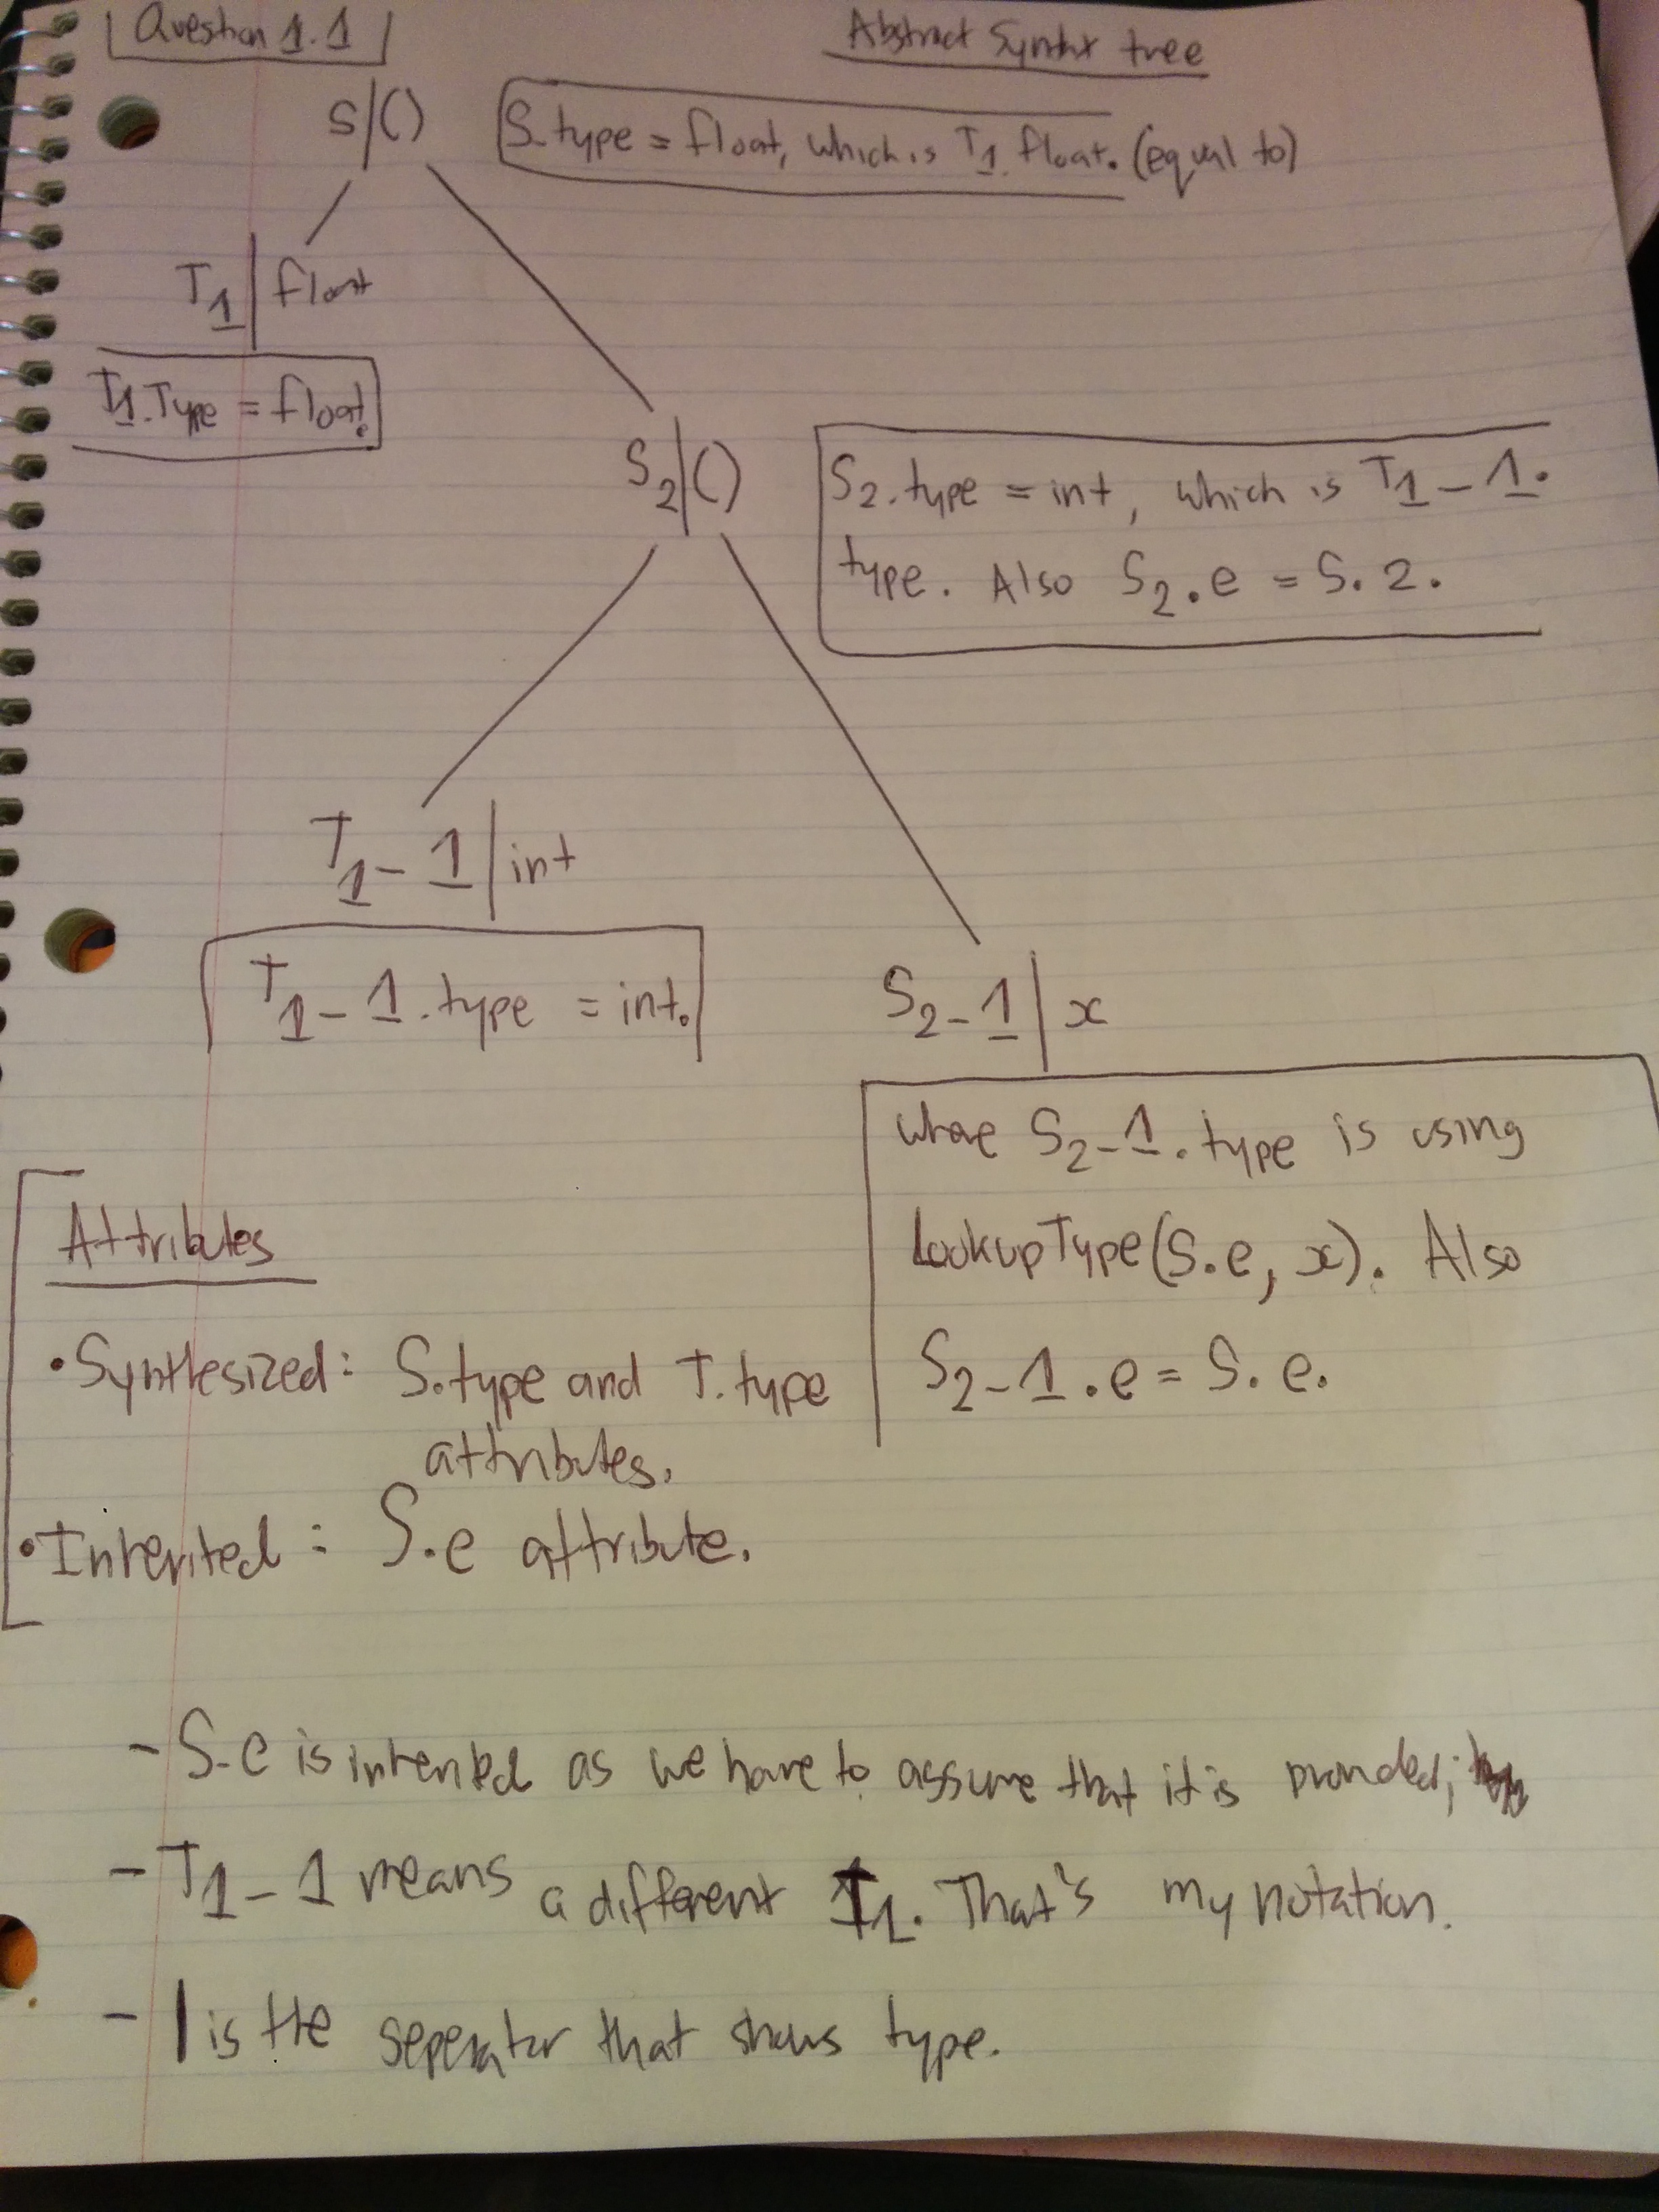
\includegraphics[scale=0.19]{IMG_20141011_142752.jpg}

\newpage

\subsection*{Question 1.2}
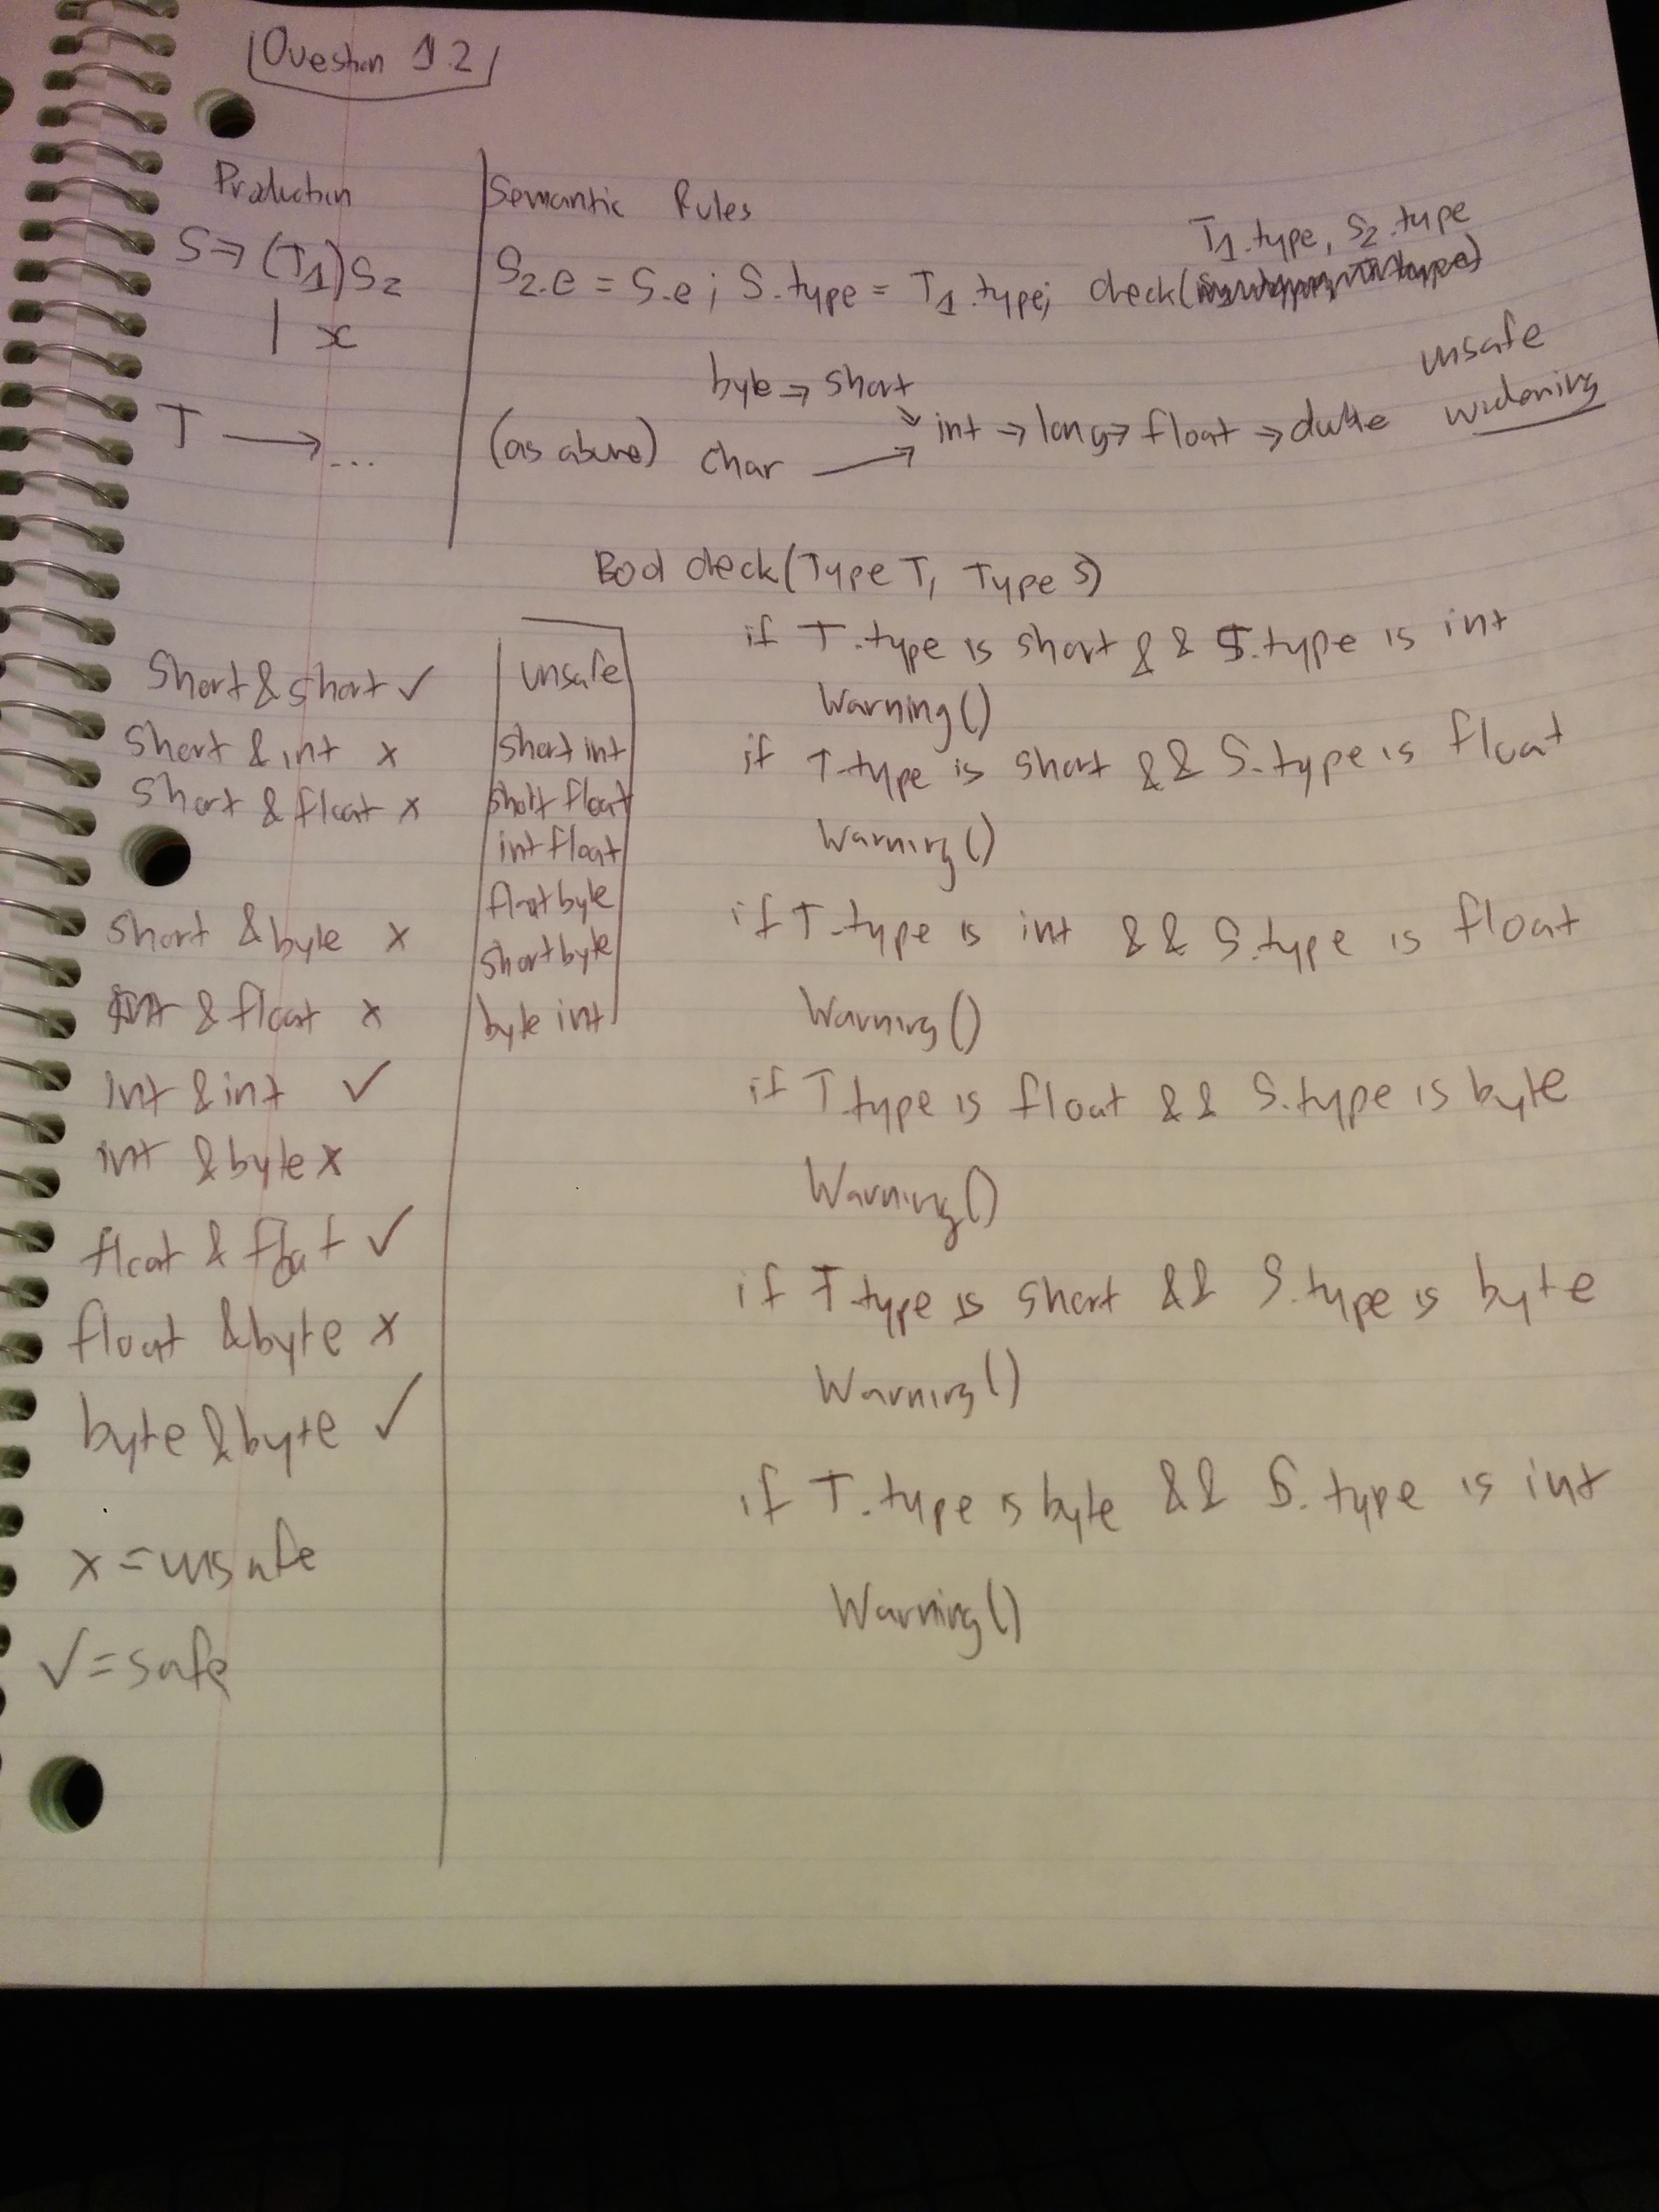
\includegraphics[scale=0.19]{IMG_20141011_211239.jpg}

\newpage

\section{Records}
\subsection*{Question 2.1}
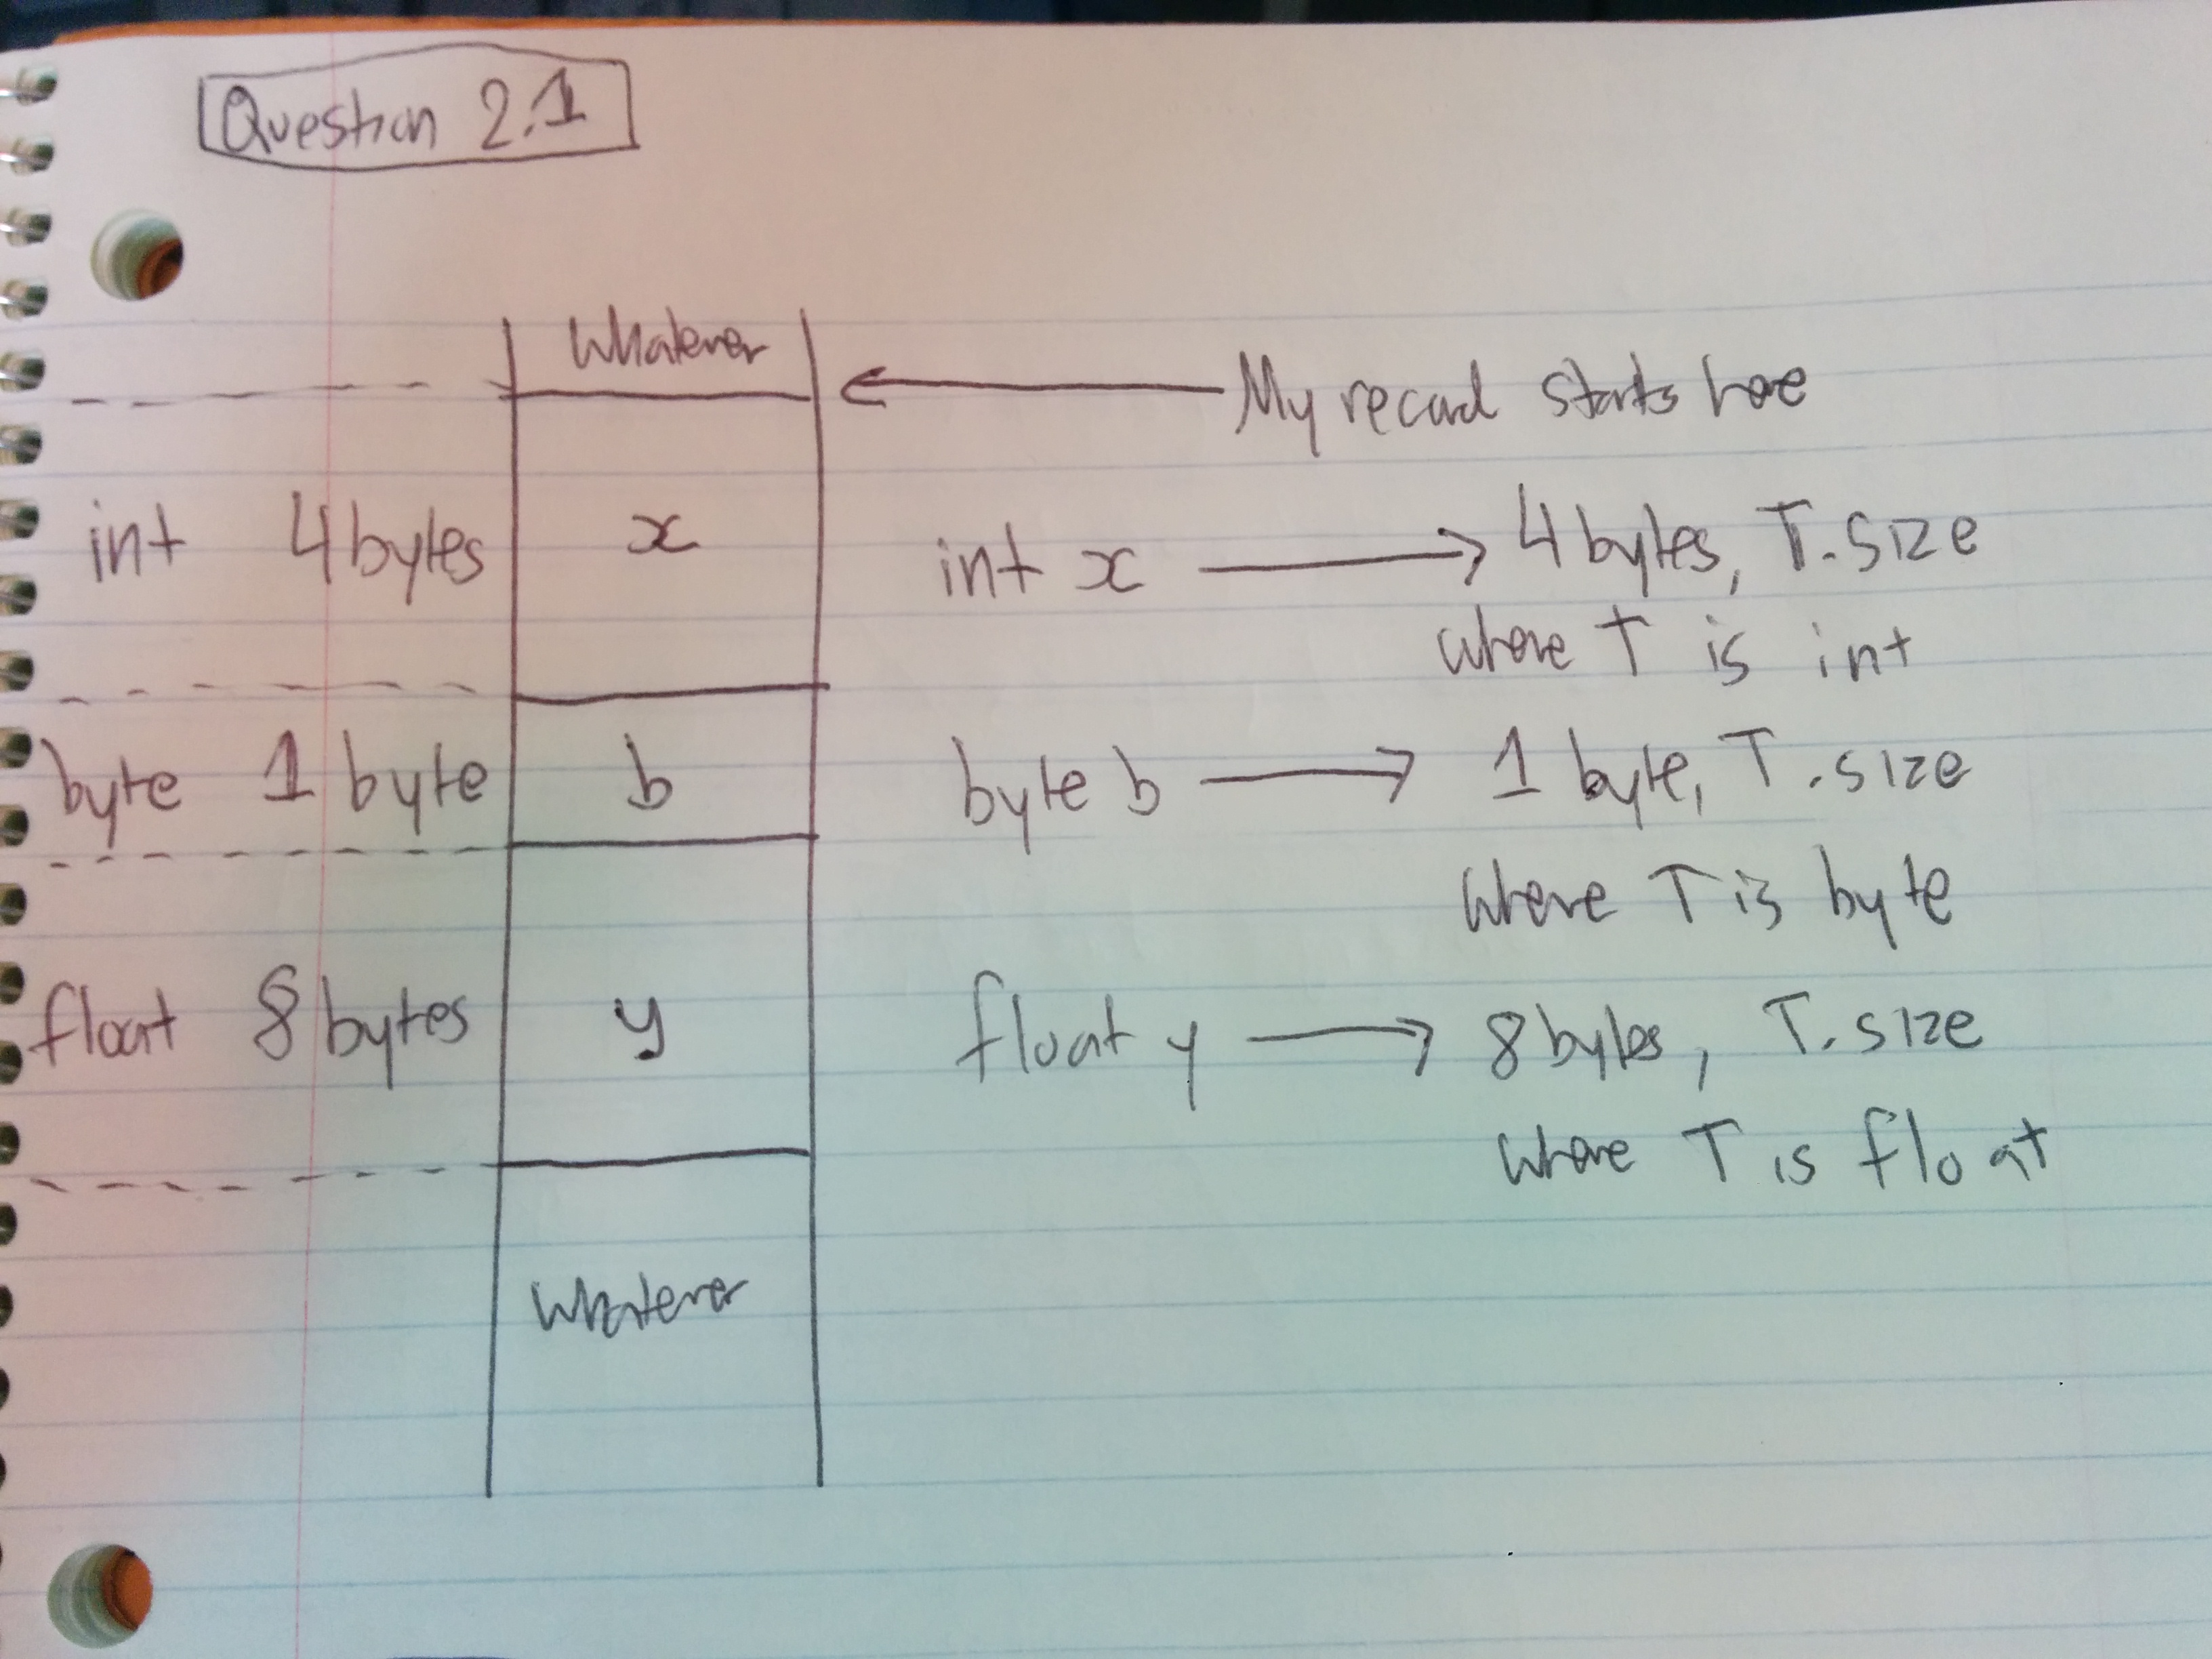
\includegraphics[scale=0.15]{IMG_20141011_151020.jpg}

\newpage

\subsection*{Question 2.2}
\par Note that there is no $;$ after $T.size$ in my correction statement. I accidentally put that in. And the missing word is $command$. Also I'd like to add my reference for page 376, which has the exact situation here.
\\
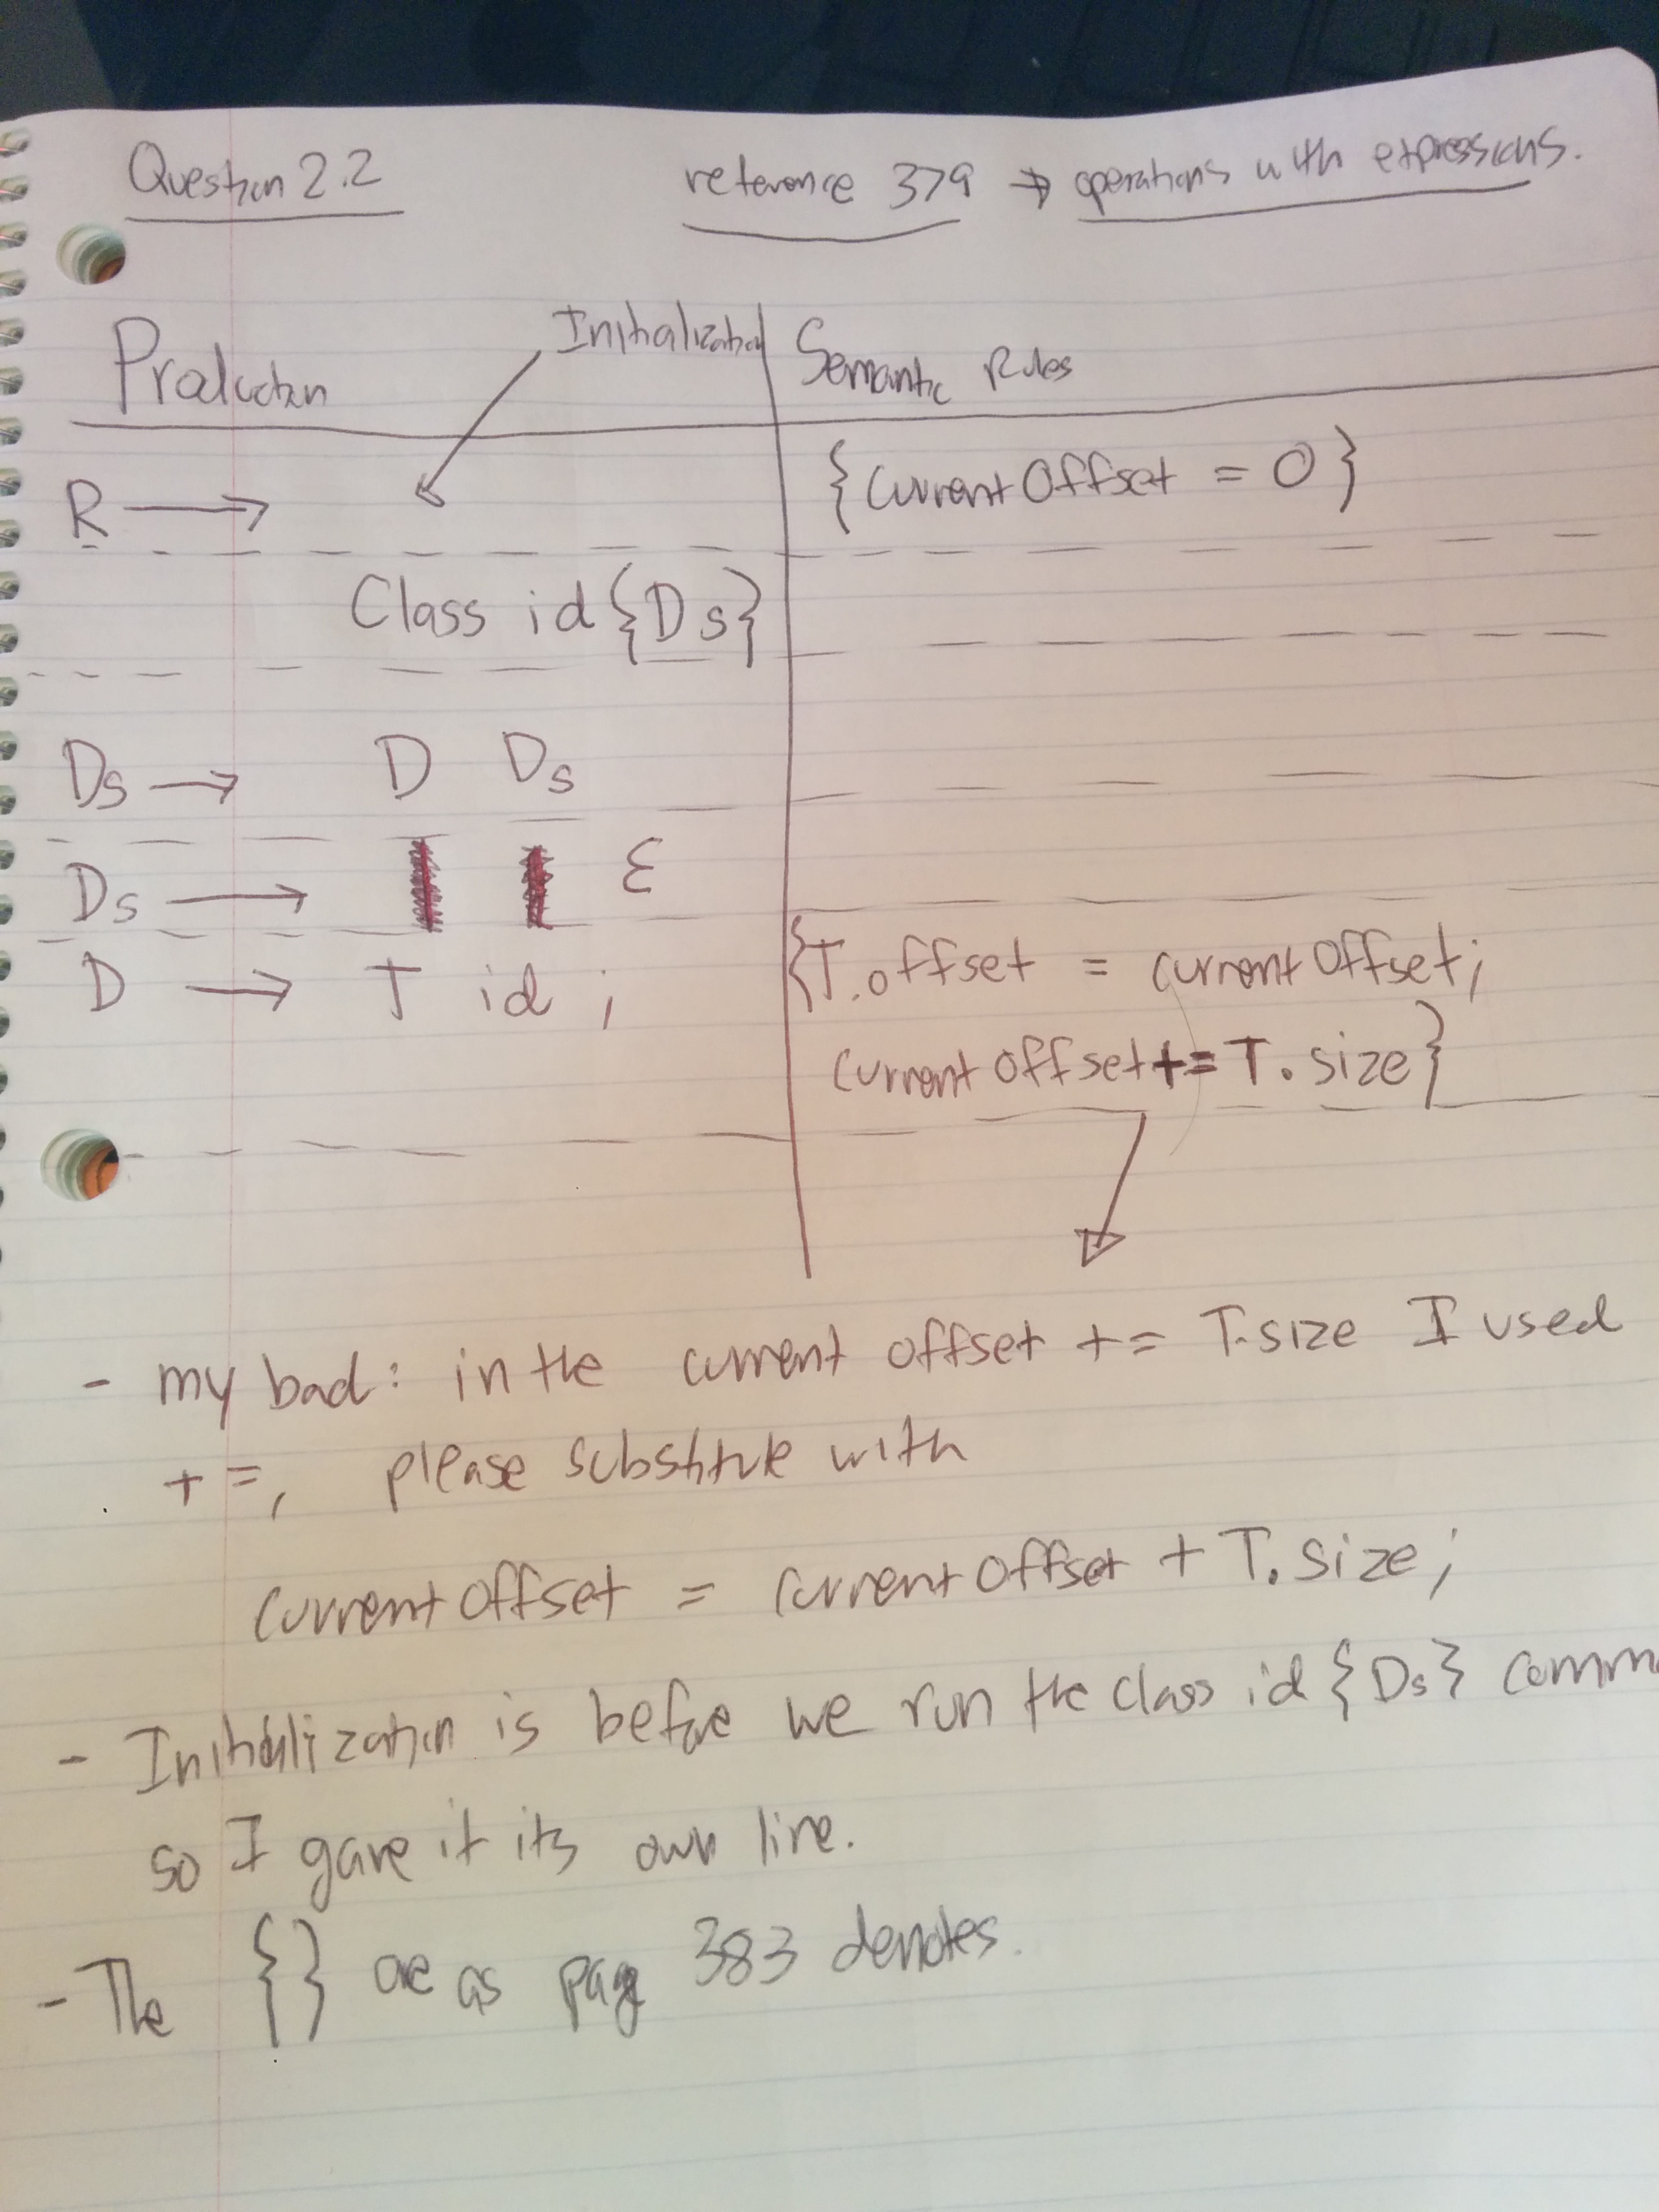
\includegraphics[scale=0.15]{IMG_20141011_154642.jpg}

\newpage

\subsection*{Question 2.3}
\par There is a \} after $+8$ that you can't see here.
\\
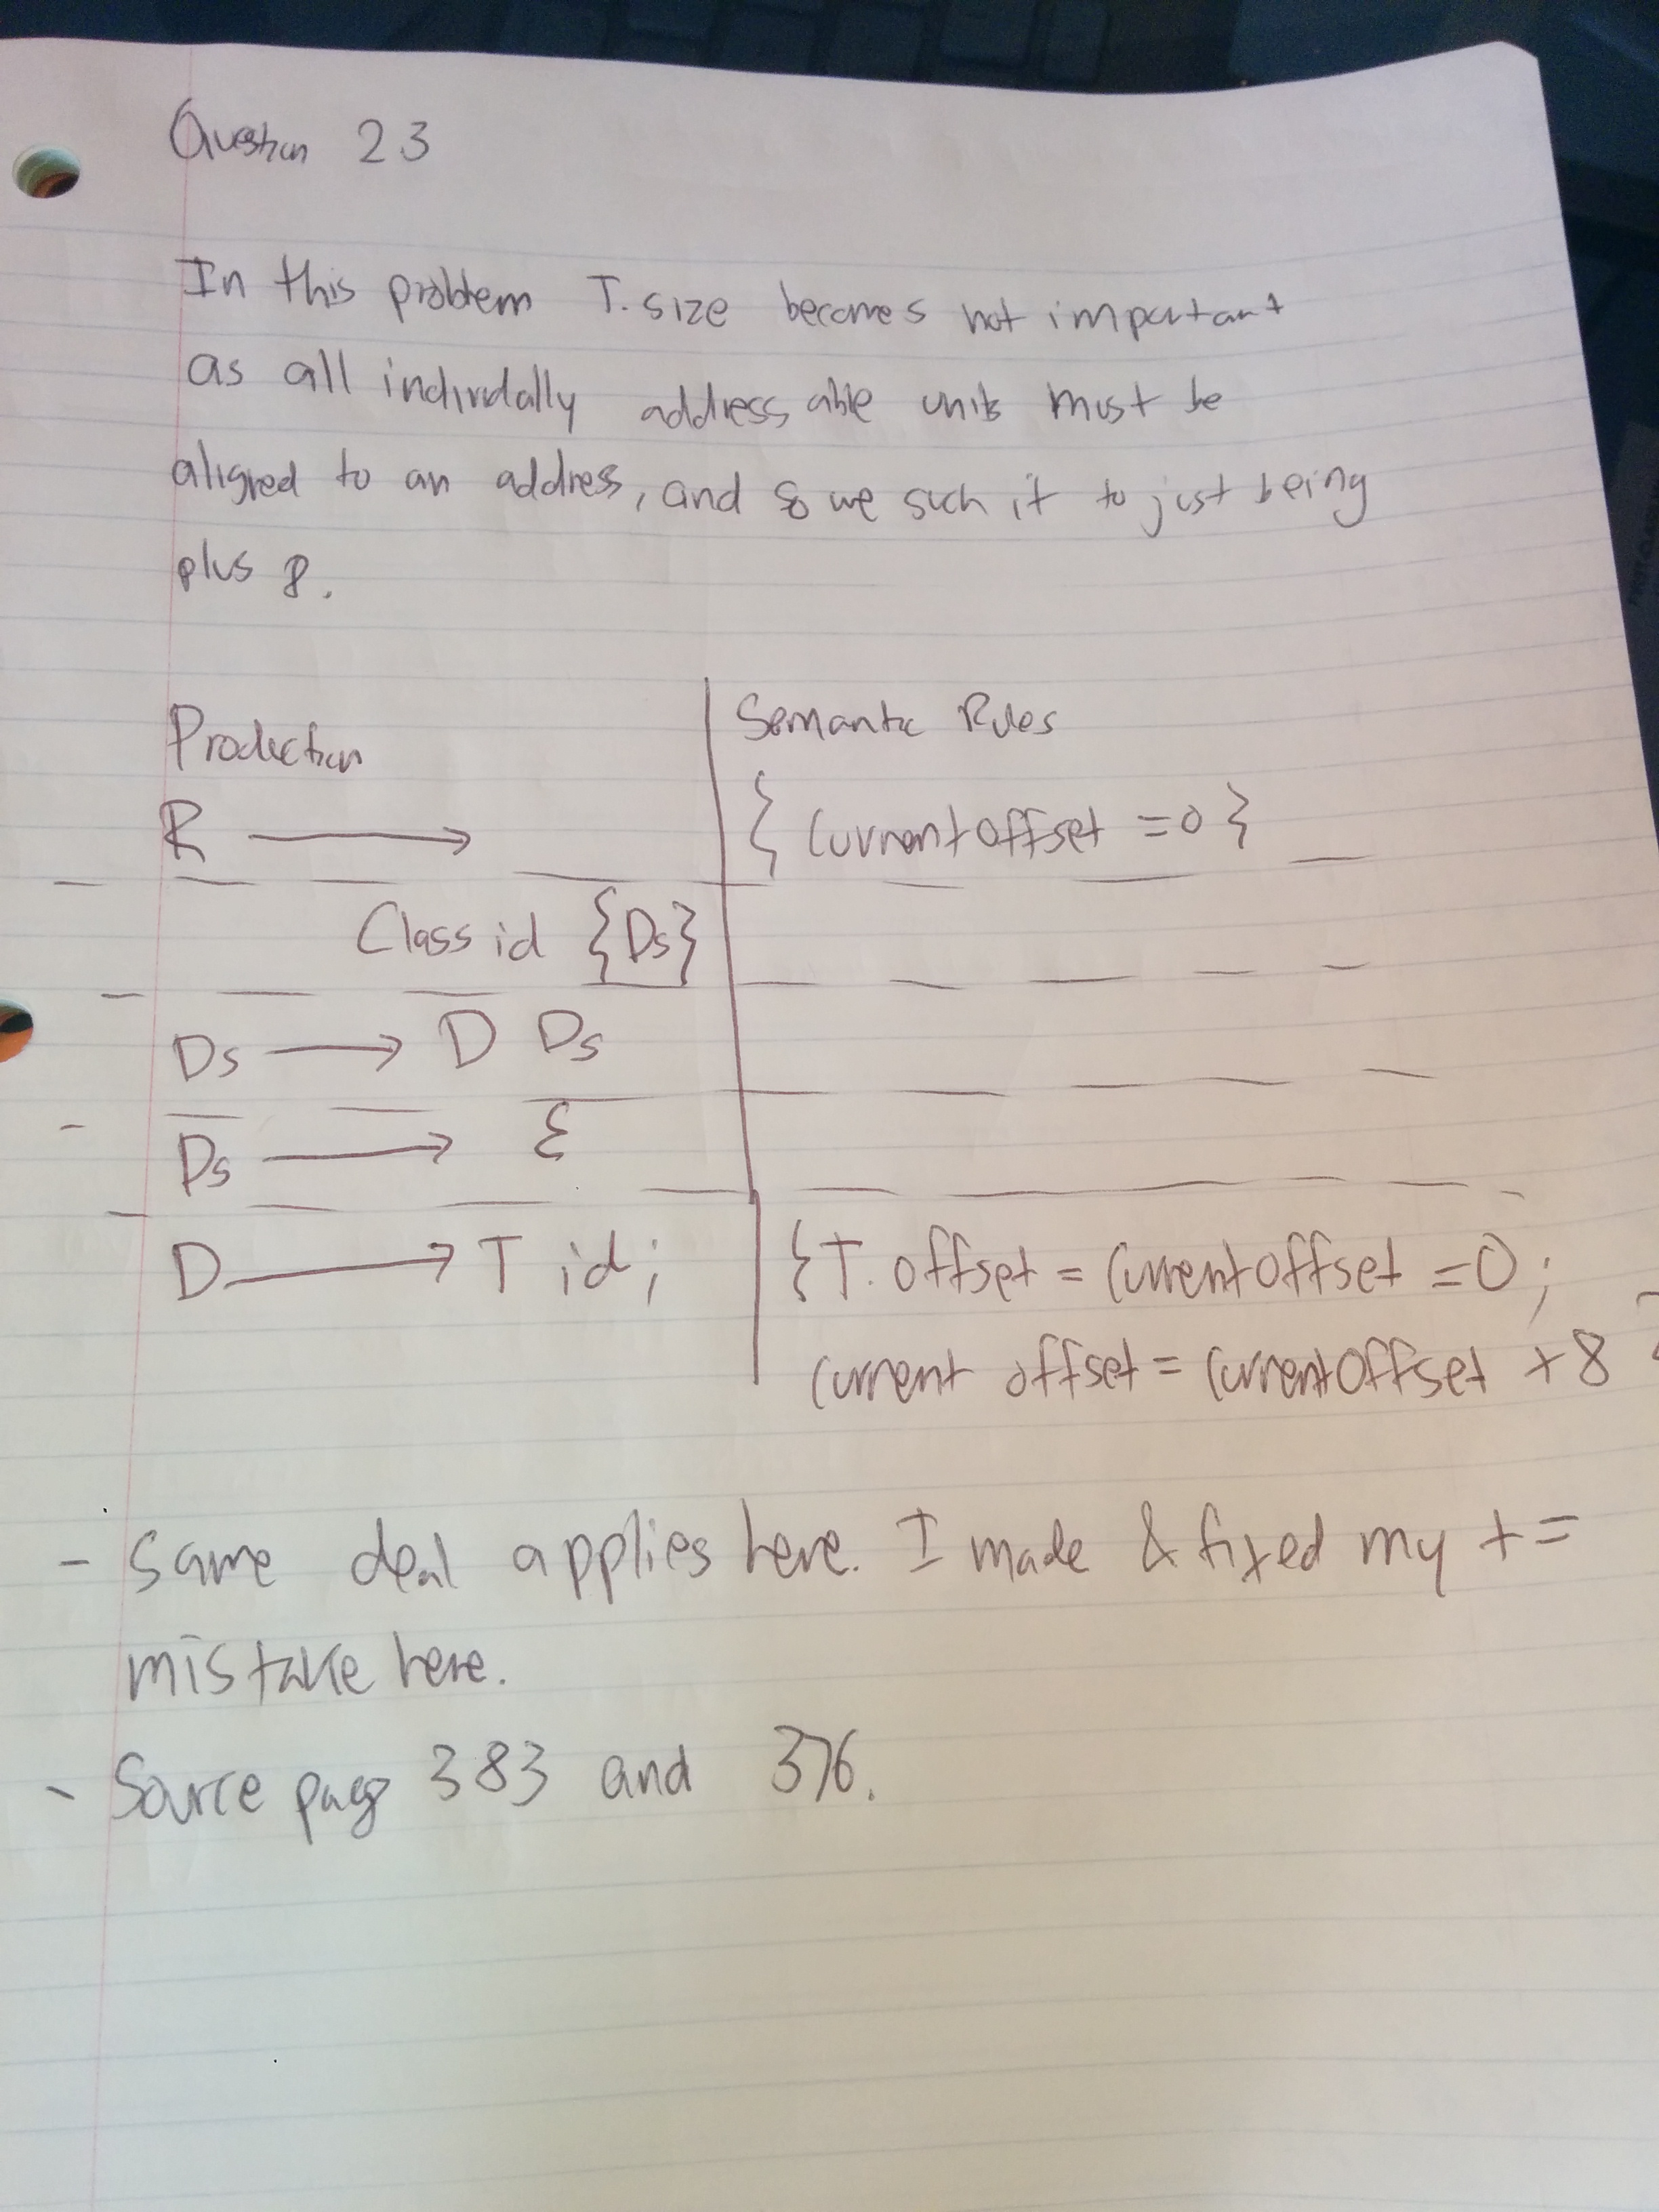
\includegraphics[scale=0.18]{IMG_20141011_155225.jpg}

\end{document}  